\documentclass[sokoban_generation_thesis.tex]{subfiles}

Jednoznaczne wyznaczenie jakości danej planszy \textit{Sokoban} jest problemem, nad którym pochylają się twórcy generujących je~metod \cite{sok_metrics} \cite{sok_metrics2} \cite{sok_metrics3}. Im~lepsza metryka oceniająca planszę, tym lepsze można dać wskazówki uczącemu się algorytmowi. Każda z~prezentowanych metod wprowadza pewien sposób szacowania jakości generowanych plansz, jednak sposoby te~są~specyficzne dla każdej metody. W~celu zestawienia wszystkich metod, wprowadza się dwie autorskie metryki, opisane poniżej.

Ludzka ocena skomplikowania planszy \textit{Sokoban} najbardziej pokrywa się z~metrykami bazującymi na~rozwiązaniu optymalnym \cite{sok_metrics}. Jak wspomniano w~p.~\ref{subs:solving_sokoban}, wyznaczenie jakiegokolwiek rozwiązania jest problemem \textit{PSPACE}-zupełnym. Mimo, że~metody takie jak SYM i~MCTS symulują rozgrywkę, dostarczając tym samym pewne rozwiązanie planszy, to~najczęściej odbiega ono istotnie od~optymalnego. Wobec tego, wartości prezentowanych metryk wyznaczane są~przy użyciu \textit{solvera} \textit{JSoko} \cite{jsoko_website}, który nie odstaje wydajnością i~skutecznością od~innych dostępnych \textit{solverów} \cite{sok_wiki}.

\begin{equation}\label{eq:psh_metric}
PSH = \frac{p}{w + h~+ b^2}
\end{equation}

Wyznaczono dwie metryki -- PSH oraz LEN, faworyzujące odpowiednio plansze wymagające dużej liczby pchnięć oraz dużej liczby ruchów gracza. Metryka opisana wyrażeniem \ref{eq:psh_metric} to~iloraz minimalnej liczby pchnięć i~sumy długości boków planszy oraz kwadratu liczby pudeł. Z~kolei druga, z~równania \ref{eq:len_metric}, to~iloraz minimalnej liczby ruchów i~iloczynu długości boków planszy.

\begin{equation}\label{eq:len_metric}
LEN = \frac{l}{w \cdot h}
\end{equation}

Metryki zostały zaprojektowane tak, by~zwracać najwyższe wyniki dla plansz uznawanych przez ludzi za~najbardziej skomplikowane. Oznacza to, że~muszą być niezależne od~rozmiarów plansz, co~zobrazowano na~rys.~\ref{rys:easy_boards}, gdzie wartości obu metryk nie przekraczają $0.5$. Żeby zobrazować zachowanie metryk dla trudniejszych plansz, na~rys.~\ref{rys:hard_board} ukazano plansze niemal trzykrotnie lepszą w~ujęciu obu z~nich.


\begin{figure}[H]
	\centering
	\begin{subfigure}[b]{0.45\textwidth}
		\centering
		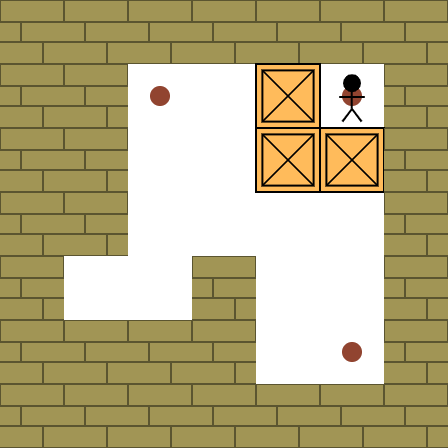
\includegraphics[width=0.8\textwidth]{board_metric5}
		\caption{$5$x$5$ - $(PSH=0.36, LEN=0.47)$}
	\end{subfigure}
	\hspace{0.02\textwidth}
	\begin{subfigure}[b]{0.45\textwidth}
		\centering
		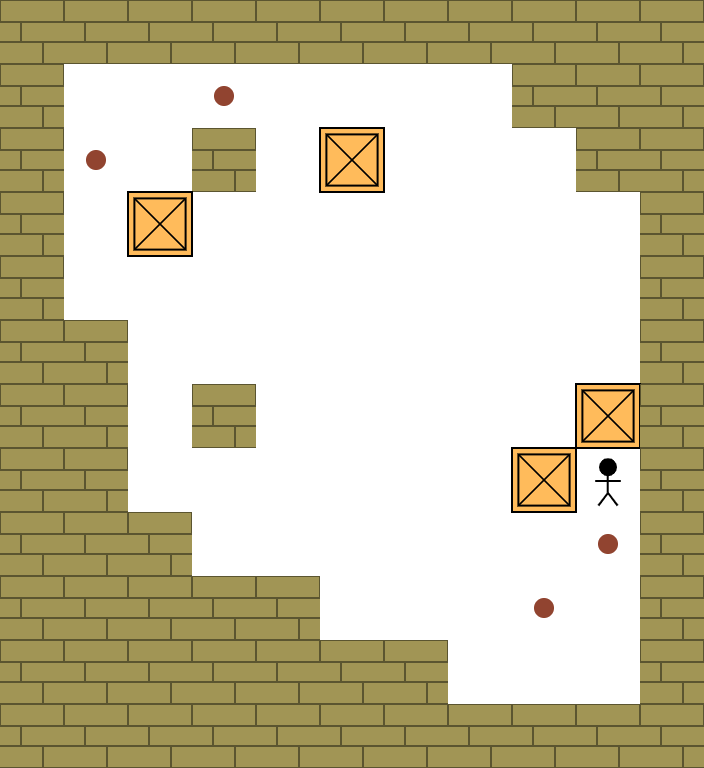
\includegraphics[width=0.8\textwidth]{board_metric10}
		\caption{$10$x$10$ - $(PSH=0.25, LEN=0.32)$}
	\end{subfigure}
	\hspace{0.02\textwidth}
	\begin{subfigure}[b]{0.45\textwidth}
		\centering
		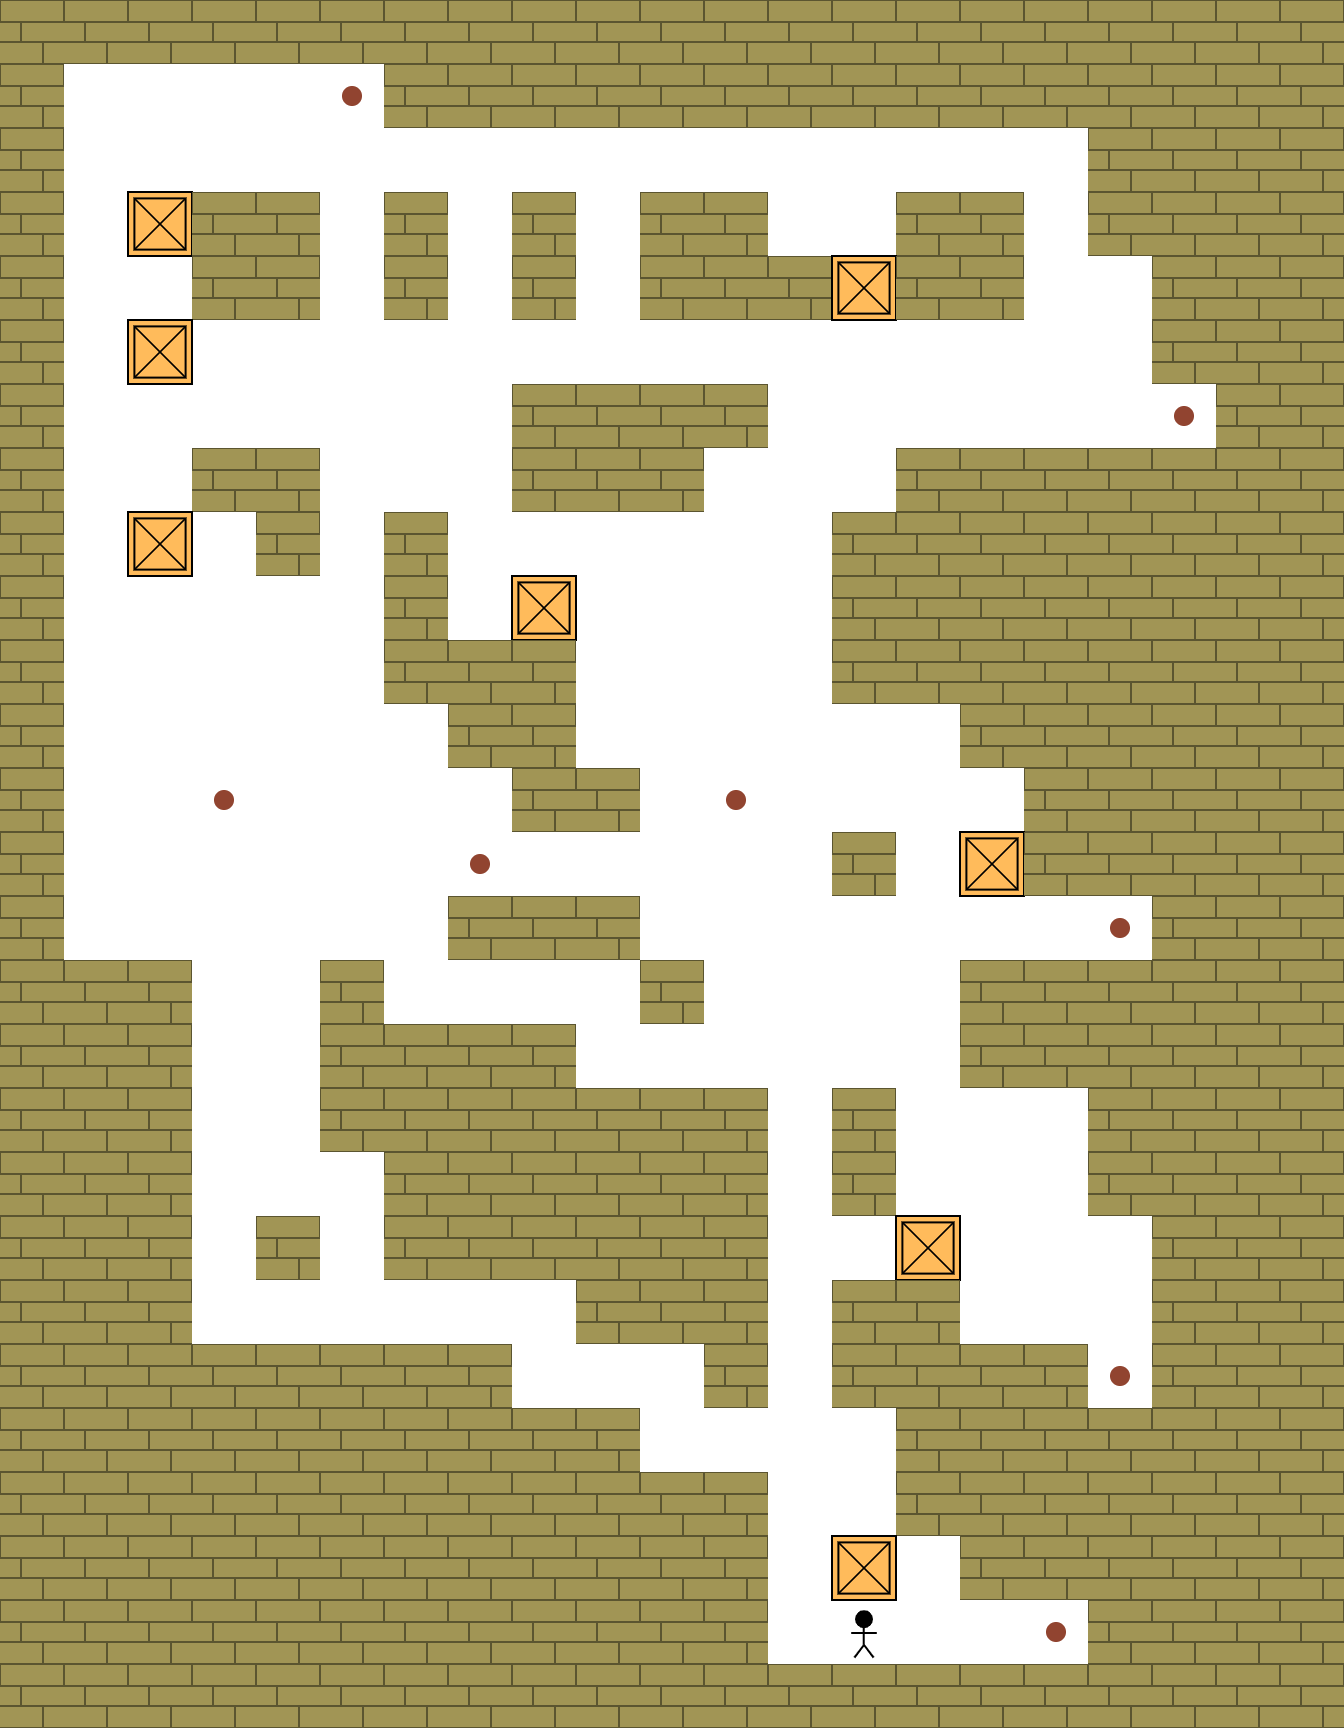
\includegraphics[width=0.8\textwidth]{board_metric25}
		\caption{$20$x$25$ - $(PSH=0.44, LEN=0.43)$}
	\end{subfigure}
	\hspace{0.02\textwidth}
	\begin{subfigure}[b]{0.45\textwidth}
		\centering
		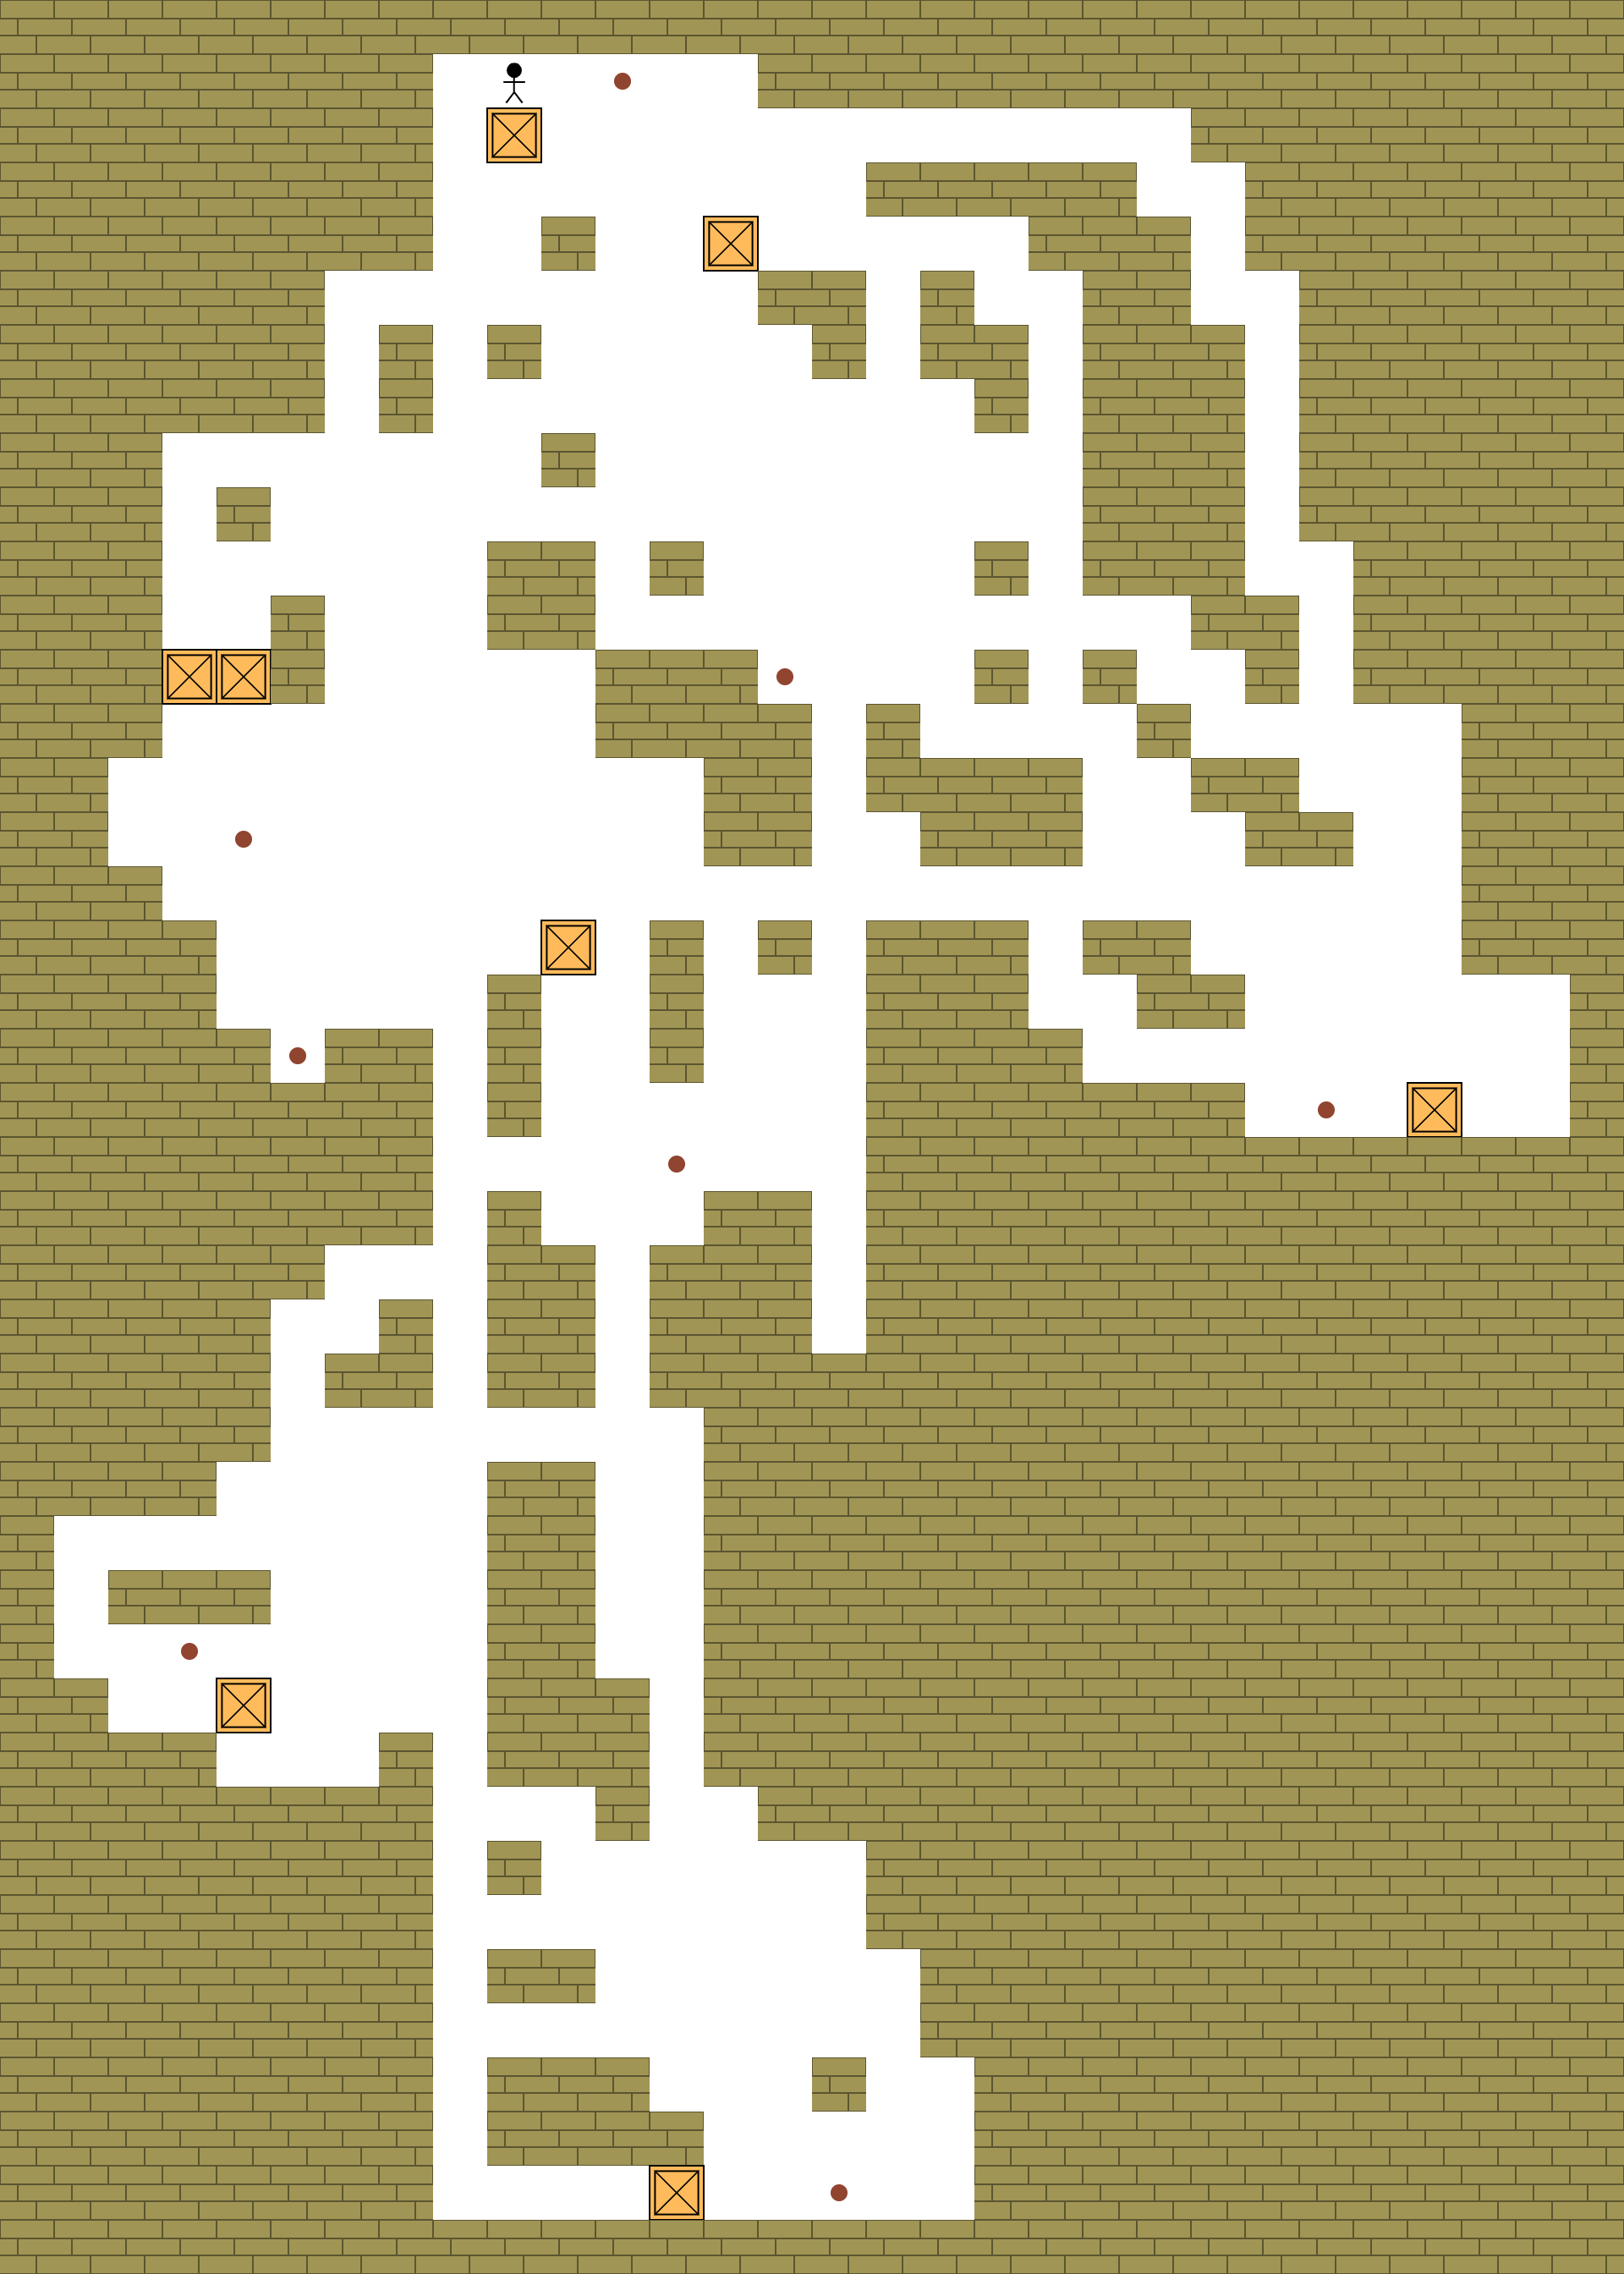
\includegraphics[width=0.8\textwidth]{board_metric40}
		\caption{$30$x$40$ - $(PSH=0.28, LEN=0.26)$}
	\end{subfigure}
	\caption{Przykłady mało skomplikowanych plansz wraz z~wartościami metryk PSH i~LEN}
	\label{rys:easy_boards}
\end{figure}

\begin{figure}[h]
	\centering
	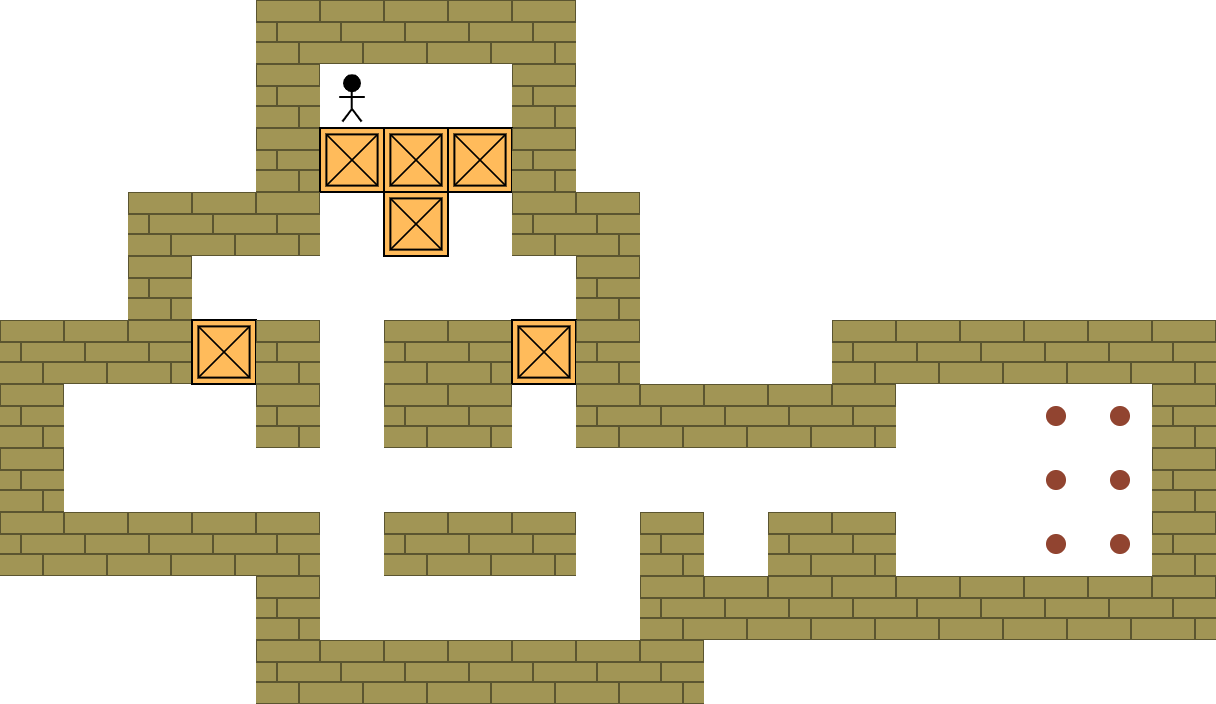
\includegraphics[width=0.5\textwidth]{board_metric_hard}
	\caption{Plansza o~wartościach metryk $(PSH=1.53, LEN=1.38)$}
	\label{rys:hard_board}
\end{figure}